\section{Put Pair Strategy}\label{sec:4}

A put gives its buyer the right to sell stock at a specified strike. Our retained pair strategy selects out-of-the-money puts near 25 delta and approximately 30 days to expiry. At delta -0.25, a small \$1 rise in the stock initially lowers the put's value by about \$0.25 per share. Delta measures price sensitivity; it is not an exact probability of exercise.


Implied volatility (IV) is the volatility input that makes an option-pricing model reproduce a quoted price. Higher IV generally means a more expensive option, holding other inputs fixed. Realized volatility (RV) describes how much the stock actually moves. Selling an option can be attractive when the premium compensates for those future movements; buying can be attractive in the opposite situation. Future RV is unknown at entry.

The pair matches initial vega and rebalances stock delta daily. Initial vega matching is a local constraint: gamma, jumps and company-specific events remain. Appendix~\ref{app:d} gives the worked contract example and Greek approximation.

\subsection{Relative Implied Volatility Signal}

For each pair, we compare the IV difference D = IV\_A - IV\_B with its latest 252 trading sessions, requiring 63 observations. At the upper quintile we sell A's relatively high-IV put and buy B's; at the lower quintile we reverse direction. Historical ranking matters: a ten-point gap means something different for a pair usually five points apart than for one usually fifteen points apart.


\begin{figure}[!htbp]\centering
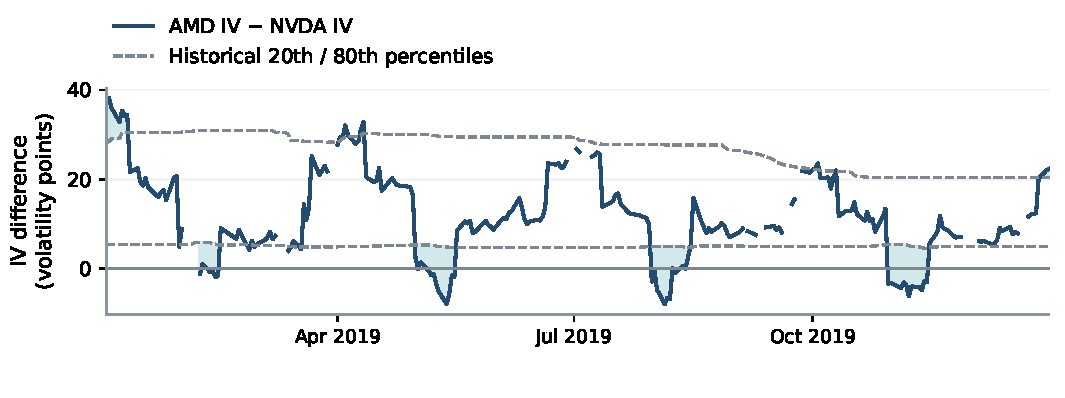
\includegraphics[width=\linewidth]{signal_example.pdf}
\caption{AMD minus NVDA selected-put IV in 2019. Shading marks excursions outside historical percentile boundaries, not executed trades. Gaps are unavailable quotes. Daily contract selection makes this a signal series, not the mark of one held contract.}\label{fig:signal-example}
\end{figure}

Monthly formation requires 126-session return beta between 0.85 and 1.15 and correlation of at least 0.5. The proposed direction must also show positive historical profit per initial vega over 91 and 365 calendar days, with 21 and 63 completed observations. These are simulated standalone candidates, not just funded fills. A trade entered yesterday with a month left cannot contribute its eventual profit today.


\subsection{Relatedness and Profitability Filters}

Beta measures the scale of one name's response to the other; correlation measures how consistently they move together. Neither guarantees that their option prices should behave alike. The relatedness screens keep the comparison among reasonably similar names without treating relatedness as the trading signal.


The profitability memory adds a different economic question: has this direction recently paid for the premium and hedging costs? We are looking for an unusually wide IV difference in a direction with evidence of structural relative richness, rather than assuming every large gap must revert. The memory and completed-count conditions are selected rules, shared across all put sizing controls.


The chart follows each day's selected contract. After entry, the simulator holds the purchased and sold contracts rather than replacing them when daily selection changes. Profit therefore depends on their realized option and hedge cash flows. A temporary narrowing of the displayed IV gap is neither required nor sufficient for a profitable expiry trade.


Entry sizing uses a regression-tree context and cross-entropy policy search. The shared sizing framework is presented in Section~\ref{sec:11}; joint performance and interpretation follow in Section~\ref{sec:results}.
\FloatBarrier
